%#!platex main

\chapter{正則表現と有限オートマトン}
\label{175712_30Mar06}

コンパイラの技法のうち、字句解析と構文解析は言語理論と関連が深い。ここで
は言語理論で用いられる用語を簡単に説明し、次いで字句解析で用いられる正則
表現と有限オートマトンについて述べる。構文解析で用いられる文脈自由文法に
ついては\ref{151253_30Mar06}章で述べる。

\section{アルファベットと記号列}

普段われわれが「文字」と呼んでいるもの
を、言語理論では{\bfseries 記号}(symbol)といい、また、記号の有限集合を
{\bf アルファベット}(alphabet)という\footnote{日常生活で英文字を
表すときに用いる「アルファベット」とは意味が異なる。}。
\begin{example}
 $\{a, b, \cdots, z\}$や$\{0, 1\}$はアルファベットである。$\Box$
\end{example}
記号が「文字」を表さないこともある。例えば、コンパイラの字句解析部では記号を
「文字」と考えてよいが、構文解析部では、記号は原始言語で意味のある文字列、
すなわちトークンである。

アルファベット$\Sigma$\footnote{アルファベットはしばしば$\Sigma$と表され
る。}中の記号からなる有限列を、$\Sigma$上の{\bf 記号列}(string)と
いう\footnote{文字列、あるいは語(word)ということもある。}。$\Sigma$上の
記号列$s$について、$s$に現れる記号の数を$s$の{\bf 長さ}といい、
$|s|$で表す。

\begin{example}
 $main$や$exercise$はアルファベット$\{a, b, \cdots, z\}$上の記号列であり、
 長さはそれぞれ$4, 8$である。また$\epsilon, 0, 11, 01011$はいずれもアルファ
 ベット$\{0, 1\}$上の記号列であり、長さはそれぞれ$0, 1, 2, 5$である。
 $\Box$
\end{example}

長さ0の記号列、つまり1つも記号を含まない記号列を{\bf 空列}(empty string)
といい、$\epsilon$という記法で表す。$|\epsilon| = 0$である。

\section{言語}

言語理論での{\bf 言語}(language)とは、日本語や英語、プログラミン
グ言語などを抽象化したものである。

アルファベット$\Sigma$上の{\bf 言語}(language)とは、$\Sigma$上の
記号列の集合である。言語に含まれる記号列は可算無限でも構わない。

\begin{example}
 $\{0\}$, $\{00, 01, 10, 11\}$, $\{1, 11, 111, 1111, \cdots\}$はいずれも
 アルファベット$\{0, 1\}$上の言語であり、それぞれ記号列$0$、長さ2のすべて
 の記号列、記号$1$のみからなるすべての記号列を表す。$\Box$
\end{example}

言語は記号列の集合であるから、空集合$\emptyset$や、空列しか含まない集合
$\{\epsilon\}$も言語である。この2 つの言語は全く異なるものであることに充
分注意しておいてほしい。$\emptyset$には要素は1つも含まれないが、
$\{\epsilon\}$には$\epsilon$という要素が1つ含まれている。

\section{言語に対する演算}

言語は(記号列の)集合であるので、$\cup,\; \cap,\; \bar{\;}$(補集合)などの
集合演算はもちろん適用できる。その他に、記号列に由来する重要な演算がいく
つかある。

\subsection{連接}

まず、{\bf 連接}という演算を紹介しよう。そのために、記号列に対する連接を定義し
ておく。2つの記号列$x, y$について、$x$の後ろに$y$が続く記号列を$x$
と$y$の{\bf 連接}(concatenation)といい、$x\cdot y$または$xy$と書
く。
\begin{example}
 $00\cdot 11 = 0011$, $111\cdot \epsilon = \epsilon\cdot 111 = 111$であ
 る。$\Box$
\end{example}

任意の記号列$x$に対して$\epsilon\cdot x = x\cdot\epsilon = x$が成り立つ。
つまり、$\epsilon$は連接に関する単位元である。

記号列$x$自身を$n$個連接した記号列を$x^n$と表し、特に
$x^0=\epsilon$と定義しておく。この結果、$i\geq 0,\, j\geq 0$に対して
$x^{i+j} = x^i\cdot x^j$が成立する。

\begin{example}
 $(01)^2 = 0101, (01)^3 = 010101$ である。$\Box$
\end{example}

さて、2つの言語$L, M$に対する連接$\cdot$を次のように定義する。
\begin{equation*}
  L\cdot M = \{s\cdot t \mid s \in L, t \in M\}
\end{equation*}
記号列の連接と同様、$\cdot$を省略して$LM$と書くこともできる。

\begin{example}
 $L = \{0, 1\}, M = \{0, 01, 111\}$とすると、
 $L\cdot M = \{00, 001, 0111, 10, 101, 1111\}$である。また
 $L \cdot \{\epsilon\} = \{\epsilon\}\cdot L = L$, 
 $M\cdot \emptyset = \emptyset \cdot M = \emptyset$である。$\Box$
\end{example}

任意の言語$L$に対し$L\cdot \{\epsilon\} = \{\epsilon\}\cdot L
= L$が成り立つ。また$L\cdot \emptyset = \emptyset\cdot L = \emptyset$が成
り立つ。つまり、言語の連接では、$\{\epsilon\}$が単位元、$\emptyset$が零元
である。

言語$L$を$n$個連接して得られる言語を$L^n$と表し、特に$L^0=\{\epsilon\}$と
する。これにより$i\geq 0,\, j\geq 0$について$L^{i+j} = L^i L^j$が成り立つ。

\subsection{閉包}

言語$L$について、次の式で定義される言語$L^\ast$を$L$の{\bfseries Kleene閉
包}(Kleene closure)という。
\[
 L^\ast = L^0 \cup L^1 \cup L^2 \cup \cdots = \bigcup_{i=0}^{\infty} L^i
\]
また次の式で定義される言語$L^+$を$L$の{\bfseries 正閉包}(positive
closure)という。
\begin{align*}
 L^+ & = L^1 \cup L^2 \cup L^3 \cup \cdots = \bigcup_{i=1}^{\infty} L^i \\
     & = L^\ast - \{\epsilon\}
\end{align*}

\begin{example}
 $L=\{a\}$とすると
 \begin{align*}
  L^0 & = \{\epsilon\} \\
  L^1 & = \{a\} \\
  L^2 & = \{aa\} \\
  L^3 & = \{aaa\} \\
  \cdots
 \end{align*}
 であり、$L^\ast = \{\epsilon, a, aa, aaa, \cdots\}$,
 $L^+ = \{a, aa, aaa, \cdots\}$である。

 また$L = \{a, b\}$とすると
 \begin{align*}
  L^0 & = \{\epsilon\} \\
  L^1 & = \{a, b\} \\
  L^2 & = \{aa, ab, ba, bb\} \\
  \cdots & 
 \end{align*}
 であり、$L^\ast = \{\epsilon, a, b, aa, ab, ba, bb, \cdots\}$, $L^+ =
 \{a, b, aa, ab, ba, bb, \cdots\}$である。この例から分かるように、各々の
 $L$から異なる要素を選んでも構わない。$\Box$
\end{example}

特に、アルファベット$\Sigma$のKleene閉包$\Sigma^\ast$
は$\Sigma$上の長さ0以上のすべての記号列からなる集合である。
\begin{align*}
 \Sigma^* & = \Sigma^0 \cup \Sigma^1 \cup \Sigma^2 \cup \cdots
\end{align*}
また$\Sigma$の正閉包$\Sigma^+$は$\Sigma$上の長さ1以上のすべての記号列か
らなる集合である。
\begin{align*}
 \Sigma^+ & = \Sigma^1 \cup \Sigma^2 \cup \cdots \\
          & = \Sigma^* - \{\epsilon\}
\end{align*}

\begin{example}
 $\Sigma = \{0, 1\}$とするとき、$\Sigma^\ast = \{\epsilon, 0, 1, 00, 01,
 10, 11, 000, \cdots\}$である。また$\Sigma^+ = \{0, 1, 00, 01, 10, 11,
 000, \cdots\}$である。$\Box$
\end{example}

\section{正則表現}

{\bfseries 正則表現}\footnote{{\bfseries 正規表現}とも言う。}(regular
expression)は、記号列の集合を簡潔に表現する記法である。まず記法の定義を
示そう。

\begin{definition}
 \label{def:regexp}
 アルファベット$\Sigma$上の正則表現とは、以下の規則から再帰的に構成される式
 である。
 \begin{enumerate}
  \item $\emptyset$は正則表現である。
  \item $\epsilon$は正則表現である。
  \item $a$(ただし$a \in \Sigma$)は正則表現である。
  \item $r,\, r'$を正則表現とするとき、$r \mid r'$は正則表現である。
	\label{182200_29Mar06}
  \item $r,\, r'$を正則表現とするとき、$r \cdot r'$は正則表現である。
	\label{182346_29Mar06}
  \item $r$を正則表現とするとき、$r^\ast$は正則表現である。
	\label{182310_29Mar06}
  \item $r$を正則表現とするとき、$(r)$は正則表現である。
	\label{182237_29Mar06}
 \end{enumerate}$\Box$
\end{definition}

\begin{example}\label{ex:regexp}
$0\cdot(0\mid 1)^\ast$はアルファベット$\{0, 1\}$上の正則表現である。なぜな
ら:
\begin{enumerate}
 \item 定義\ref{def:regexp}の\ref{182015_29Mar06}により$0,\, 1$はそれぞれ正
       則表現である。
 \item 定義\ref{def:regexp}の\ref{182200_29Mar06}により$0 \mid 1$は正則表
       現である。
 \item 定義\ref{def:regexp}の\ref{182237_29Mar06}により$(0 \mid 1)$は正則
       表現である。
 \item 定義\ref{def:regexp}の\ref{182310_29Mar06}により$(0 \mid 1)^\ast$は正
       則表現である。
 \item 定義\ref{def:regexp}の\ref{182346_29Mar06}により$0\cdot(0 \mid 1)^\ast$は
       正則表現である。
\end{enumerate}$\Box$
\end{example}

アルファベット$\Sigma$上の正則表現は、$\Sigma$上のある言語を表している。

\begin{definition}
 アルファベット$\Sigma$上の正則表現$R$の表す言語$L(R)$は、以下のように再
 帰的に定義される。
 \begin{enumerate}
  \item $L(\emptyset) = \emptyset$
  \item $L(\epsilon) = \{\epsilon\}$
  \item $L(a) = \{a\}$
	\label{182015_29Mar06}
  \item $r,\, r'$の表す言語をそれぞれ$L(r),\, L(r')$とするとき、
	$L(r \mid r') = L(r) \cup L(r')$
  \item $r,\, r'$の表す言語をそれぞれ$L(r),\, L(r')$とするとき、
	$L(r \cdot r') = L(r) \cdot L(r')$
  \item $r$の表す言語を$L(r)$とするとき$L(r^*) = L(r)^*$
  \item $r$の表す言語を$L(r)$とするとき$L((r)) = L(r)$
 \end{enumerate}$\Box$
\end{definition}

\begin{example}
 例\ref{ex:regexp}の正則表現は言語$\{0, 00, 01, 000, 001, 010, 011, 0000, \cdots\}$、つま
 り、0の後ろに0と1が0個以上続くような記号列全体を表している。なぜなら:
 \begin{align*}
 L(0\cdot (0\mid 1)^\ast) & = L(0) \cdot L((0 \mid 1)^\ast) \\
                 & = L(0) \cdot L((0 \mid 1))^\ast \\
                 & = L(0) \cdot L(0 \mid 1)^\ast \\
                 & = L(0) \cdot (L(0) \cup L(1))^\ast \\
                 & = \{0\} \cdot \{0, 1\}^\ast \\
                 & = \{0\} \cdot \{\epsilon, 0, 1, 00, 01, 10, 11, \cdots\} \\
                 & = \{0, 00, 01, 000, 001, 010, 011, \cdots\}
 \end{align*}$\Box$
\end{example}

正則表現に用いられる演算子$\ast,\;\cdot,\;\mid$の優先順位は、$\ast$が最も
高く、ついで$\cdot$、最も低いのが$\mid$となる。また$r\cdot r'$は$rr'$と書
いてもよい。

以降、正則表現に関して次の略記法を用いることがある。
\begin{align*}
 r^+ & \equiv rr^\ast \\
 r? & \equiv r \mid \epsilon \\
 [abc] & \equiv a \mid b \mid c \\
 [a\,\mbox{-}\,z] & \equiv a \mid \cdots \mid z
\end{align*}

\begin{example}
 C言語の10進定数は0以外の数字で始まり、その後に0個以上の数字が続くので、正則表現
$[1\,\mbox{-}\,9]\,[0\,\mbox{-}\,9]^\ast$で表せる(練習問題\ref{ex:regexp_03},
\ref{ex:regexp_04}, \ref{ex:regexp_05}参照)。$\Box$
\end{example}

\section{有限オートマトン}

正則表現は、{\bfseries 有限オートマトン}(finite automaton)という計算モ
デルと極めて関連が深い。

\begin{figure}
 \begin{center}
  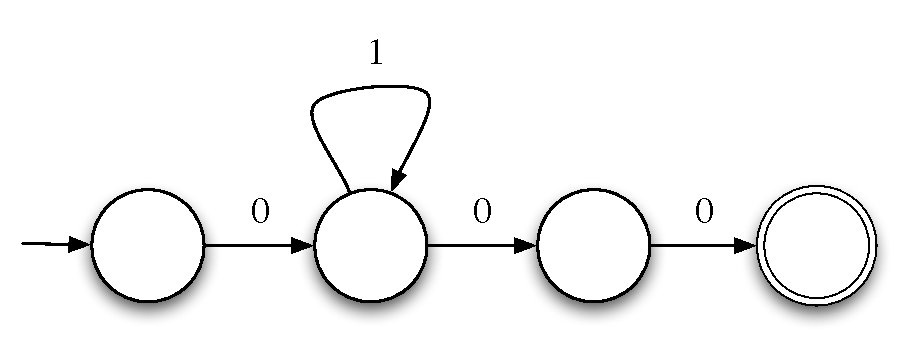
\includegraphics[width=12cm]{figure/finite_automaton.pdf}
 \end{center}
 \caption{有限オートマトン}
 \label{162900_30Mar06}
\end{figure}

直観的には、有限オートマトンはいくつかの{\bfseries 状態}(state)と状態間
の{\bfseries 遷移}(transition)からなる有向グラフで表される(図
\ref{162900_30Mar06})。状態には1つの{\bfseries 初期状態}(initial state)、
複数個の{\bfseries 受理状態}(accepting state)があり、また、各遷移には
アルファベット中の1文字(ラベル)が付けられている。最初、有限オートマトンは初期状態に制御がある。そし
て、入力を1文字読むごとに、入力を現在制御が置かれている状態から伸びる遷移
のラベルと照合し、合致する遷移先の状態に制御を移す。このように状態間の遷
移を繰り返し、入力を読み切ったときに受理状態に制御があれば、その入力を受
理する。図\ref{162900_30Mar06}の有限オートマトンは、0で始まり、次に1が0個
以上続き、00で終わるような記号列をすべて受理する。なお、以下では、
$\epsilon$をラベルに持つ遷移はなく、かつ各状態について、入力となる記号と
照合される遷移は常に1つだけであると仮定する\footnote{すなわち、ここで考え
る有限オートマトンは{\bfseries 決定性}(deterministic)であると仮定す
る。}。

\begin{definition}
 (決定性)有限オートマトン$A$は5つ組$(Q, \Sigma, \delta, q_0, F)$である。
 ここで、
 \begin{itemize}
  \item $Q$:状態の有限集合
  \item $\Sigma$:入力記号の有限集合
  \item $\delta$:遷移関数(transition function)。状態と入力記号を与える
	と状態1つを返す
  \item $q_0 \in Q$:初期状態
  \item $F \subseteq Q$:受理状態の集合
 \end{itemize}$\Box$
\end{definition}

% 有限オートマトンの例

実は、正則表現と有限オートマトンは等価\footnote{任意の正則表現に対して、
その表す言語を受理する有限オートマトンが存在する。また、任意の有限オート
マトンに対して、それが受理する言語を表す正則表現が存在する。}であり、任意
の正則表現から等価な有限オートマトンを構成したり、任意の有限オートマトン
から等価な正則表現を構成することができる。手法の詳細は別の書籍を参照され
たい(例えば\cite{ホップクロフト03:automaton})。この講義で必要になるのは、
極めて簡単な形式の正則表現から有限オートマトンを構成することだけなので、
これについて直観的な説明をするにとどめる。

基本的な正則表現について、対応する有限オートマトンは図
\ref{125936_30Mar06}のようになる。これを再帰的に用いて、有限オートマトン
を順に構成し、最後に初期状態と受理状態を定めればよい。ただし$\epsilon$の
扱いは注意が必要である。$\epsilon\cdot a = a\cdot\epsilon = a$などの性質
を用いて、あらかじめ正則表現から$\epsilon$を除去し、有限オートマトンを構
成しなければならない\footnote{$\epsilon$については、この方法ではうまくい
かない場合があるかもしれない。厳密には、正則表現$\rightarrow$ $\epsilon$
遷移つき非決定性有限オートマトン $\rightarrow$ 非決定性有限オートマトン
$\rightarrow$ 決定性有限オートマトンの順に変換を行わなければならない。詳
細は\cite{ホップクロフト03:automaton}などを参照されたい。}。

\begin{figure}
 \begin{center}
  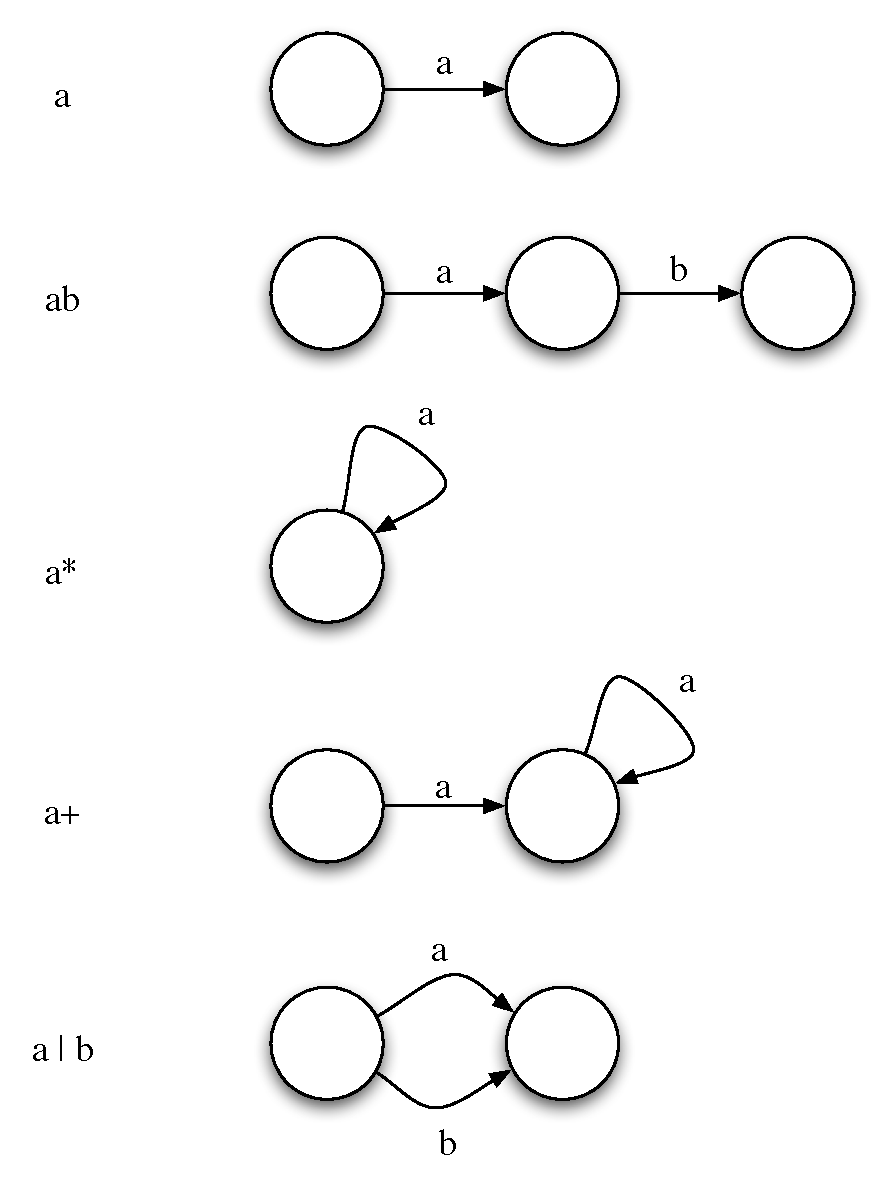
\includegraphics[width=12cm]{figure/regexp_and_fa.pdf}
 \end{center}
 \caption{正則表現と対応する有限オートマトン}
 \label{125936_30Mar06}
\end{figure}

\section{練習問題}

\begin{exercise}
 \label{ex:regexp_01}
 次の言語を表す正則表現を示せ。
 \begin{enumerate}
  \item アルファベット$\{0, 1\}$上の記号列のうち、0から始まり1が0回以上続
	くもの全体からなる言語
  \item アルファベット$\{a, b, c\}$上の記号列のうち、1個以上の$a$と1個以
	上の$b$を含むもの全体からなる言語
  \item アルファベット$\{0, 1\}$上の記号列のうち、0と1が交互に出現するも
	の全体からなる言語
 \end{enumerate}
\end{exercise}
\begin{exercise}
 \label{ex:regexp_02}
 正則表現 $(0 \mid 1)^\ast 0(0\mid 1)(0\mid 1)$ が表す言語は何か。言葉で説明せよ。
\end{exercise}
\begin{exercise}
 \label{ex:regexp_03}
 C言語の空白記号は、空白($_{\sqcup}$)、タブ(\verb|\t|)、改行
 (\verb|\n|)が1個以上並んだ文字列である。これを正則表現で表せ。
\end{exercise}
\begin{exercise}
 \label{ex:regexp_04}
 C言語の16進定数は 0x あるいは 0X で始まり、数字および a, b, c, d, e, f,
 A, B, C, D, E, F が1個以上続く。これを正則表現で表せ。
\end{exercise}
\begin{exercise}
 \label{ex:regexp_05}
 C言語の識別子はA〜Z, a〜z, 0〜9, 下線(\underline{ })からなる文字列であ
 る。ただし、最初の文字に数字を使うことはできない。これを正則表現で表せ。
\end{exercise}
\begin{exercise}
 \label{ex:regexp_06}
 アルファベットを$\{0, 1\}$とするとき、次の言語を受理する有限オートマト
 ンを示せ。
 \begin{enumerate}
  \item $00$で終わる記号列全体
  \item $011$を途中に含む記号列全体
 \end{enumerate}
\end{exercise}
\begin{exercise}
 \label{ex:regexp_07}
 正則表現$00(0 \mid 1)^\ast$に対応する有限オートマトンを構成せよ。
\end{exercise}
